\chapter{Аналитическая часть}
В данном разделе рассмотрены анализ задач отображения объектов, построения реалистичных изображений, генерации местности. Кроме того, рассматриваются методы решения вышеуказанных задач.

\section{Описание объектов}

\subsection{Типы моделей}
Существует несколько типов геометрической модели тела. Ниже представлены их описание и сравнение.

\subsubsection{Каркасная модель}
Каркасная модель является наиболее примитивным типом модели тела. Представляет собой набор вершин и ребер, без учета материала и характеристик граней/поверхностей тела. Получаемые в результате применения каркасных моделей изображения неоднозначны: нет возможности автоматизировать процессы удаления невидимых линий \cite{bib:10}.

\subsubsection{Поверхностная модель}
Поверхностная модель, в отличие от каркасной, позволяет описывать поверхности тела, в том числе аналитическим способом, но не учитывает направление поверхности. Таким образом, не производится учет внешних/внутренних поверхностей тела.

\subsubsection{Объемная модель}
Объемная модель является модификацией поверхностной модели с тем отличием, что предоставляет информацию  о направлении поверхности и расположении материала относительно поверхностей. Таким образом, становится возможным учет внутренней структуры тела. Объемные модели позволяют описывать объекты с большой степенью точности.

\subsubsection{Выбор типа модели}
В результате анализа и сравнения типов моделей, было решено использовать поверхностную модель, так как она позволяет оперировать поверхностями и текстурами объекта, при этом в данной задаче нет необходимости в анализе внутренней структуры тел.

\subsection{Способы задания модели}
\subsubsection{Аналитический}
Модель задается с помощью аналитический выражений (уравнений) \cite{bib:4} вида

\begin{equation}
	f(x, y, z) = 0.
\end{equation}

Кроме явного уравнения, часто используется параметрическая форма вида $x = x(t)$.

Основными особенностями такого способа задания модели является высокая производительность по времени, отсутствие дополнительных затрат памяти, сложность преобразований, сложность задания высокодетализированных объектов в аналитической форме.

Аналитический способ используется в основном для задания простых объектов, например, ограниченных поверхностями второго порядка.

\subsubsection{С использованием полигональной сетки}
Полигональная сетка~---~это поверхность, заданная как множество полигонов \cite{bib:5}. Она представляет собой набор вершин, связей между ними (ребер) и граней. Эти составляющие и описывают форму объекта.

Среди особенностей полигональной сетки можно отметить то, что с помощью нее можно отображать любые поверхности~---~разбивая ее на маленькие объекты (полигоны). Благодаря этому, полигональная сетка используется в большинстве сфер применения компьютерной графики, например, в компьютерных играх. Кроме того, стоит отметить большой объем требуемой памяти из-за необходимости хранить все полигоны, и низкая производительность. Например, для хранения сферы аналитическим способом достаточно хранить центр и радиус, при этом при данном способе необходимо хранить информацию о всех полигонах сферы, которых может быть несколько тысяч.

\subsubsection{Выбор способа задания модели}
В рамках данной задачи, необходимо строить сложные объекты~---~деревья, а также генерировать их, то есть преобразование сгенерированных данных в уравнения не представляется возможным. Поэтому был выбран способ задания модели с использованием полигональной сетки, как полностью удовлетворяющий требованиям данной задачи.

\section{Составляющие сцены}
Сцена состоит из следующих составляющих.

\begin{itemize}
	\item Модель, заданная с использованием полигональной сетки. Модель характеризуется следующими параметрами:
	\begin{itemize}
	    \item координатами вершин;
	    \item списком полигонов;
	    \item цветом материала;
	    \item цветом бликов;
	    \item коэффициентом диффузного отражения;
	    \item коэффициентом зеркального отражения;
	    \item коэффициентом фонового освещения.
	\end{itemize}
	\item Камера, которая характеризуется следующими параметрами:
	\begin{itemize}
	    \item координатами;
	    \item направлением взгляда.
	\end{itemize}
	\item Источник света, который характеризуется следующими параметрами:
	\begin{itemize}
	    \item координатами;
	    \item интенсивностью освещения.
	\end{itemize}
\end{itemize}

\section{Построение реалистичного изображения}
Важнейшей частью работы является построение реалистичного изображения сгенерированной местности. 

Основными этапами синтеза реалистичного изображения являются \cite{bib:7}:

\begin{itemize}
	\item разработка трехмерной математической модели синтезируемой визуальной обстановки;
	\item определение направления линии визирования , положения картинной плоскости, размеров окна обзора, значений управляющих сигналов;
	\item формирование операторов, осуществляющих пространственное перемещение моделируемых объектов визуализации;
	\item преобразование модели, синтезируемой в пространстве, к координатам наблюдателя;
	\item отсечение объектов визуального пространства в пределах пирамиды видимости;
	\item вычисление двумерных перспективных проекций синтезируемых объектов видимости на картинную плоскость;
	\item исключение невидимых элементов синтезируемого пространства при данном положении наблюдателя, закрашивание и затенение видимых элементов объектов визуализации;
	\item вывод полутонового изображения синтезируемого визуального пространства на экран растрового дисплея.
\end{itemize}

\subsection{Удаление невидимых линий и поверхностей}
Существует множество алгоритмов удаления невидимых линий и поверхностей, которые разделяются на две категории \cite{bib:7}:

\begin{itemize}
	\item Алгоритмы, работающие в объектном пространстве~---~имеют дело с физическими координатами, в которых описаны исходные объекты. Имеют высокую точность, однако неэффективны по времени, поэтому используются в основном для несложных сцен \cite{bib:7}.
	\item Алгоритмы, работающие в пространстве изображения~---~имеют дело с координатами экрана. Точность ограничена разрешением дисплея. Но за счет большей эффективности используются для отрисовки более сложных сцен, чем алгоритмы, работающие в объектном пространстве.
\end{itemize}

В рамках данной задачи будет производится отрисовка сцен с большим количеством объектов, поэтому наиболее целесообразным является использование алгоритмов, работающих в пространстве изображения.

\subsubsection{Алгоритмы разбиения на окна}

Данные алгоритмы используют гипотезу о том, что на обработку областей, содержащих мало информации, мозгом человека тратится мало времени \cite{bib:8}. Далее дано описание алгоритма.

\begin{enumerate}
\item В пространстве изображения рассматривается окно, и решается вопрос о том, есть ли в этом окне объекты, и достаточно ли оно простое для визуализации. Если оно не является достаточно простым, то происходит дальнейшее разбиение на подокна, пока они не станут достаточно простыми. Разбиение ограничено точностью растрового дисплея.

 \item При достижении достаточно простого для визуализации окна, часто окна размером в один пиксел, необходимо выбрать один из вариантов алгоритмов: удаления невидимых линий и удаления невидимых поверхностей \cite{bib:8}:
 
 \begin{itemize}
 
 \item при удалении невидимых линий, пиксел закрашивается цветом линии, если через него проходит какая-либо линия, иначе, закрашивается фоновым цветом;
 
 \item при удалении невидимых поверхностей, происходит проверка охвата пиксела многоугольниками сцены. Если пиксел охвачен какими-либо многоугольниками, то выбирается ближайший относительно центра пиксела многоугольник, и пиксел закрашивается в его цвет. Иначе, если пиксел не охвачен каким-либо многоугольником, он закрашивается цветом фона.

 \end{itemize}
 
 \end{enumerate}
 
 Процесс разбиения на подокна образует древовидную структуру, показанную на рис.~\ref{img:windows}.
 
\noindent
\begin{figure}[h!]
	\centering
    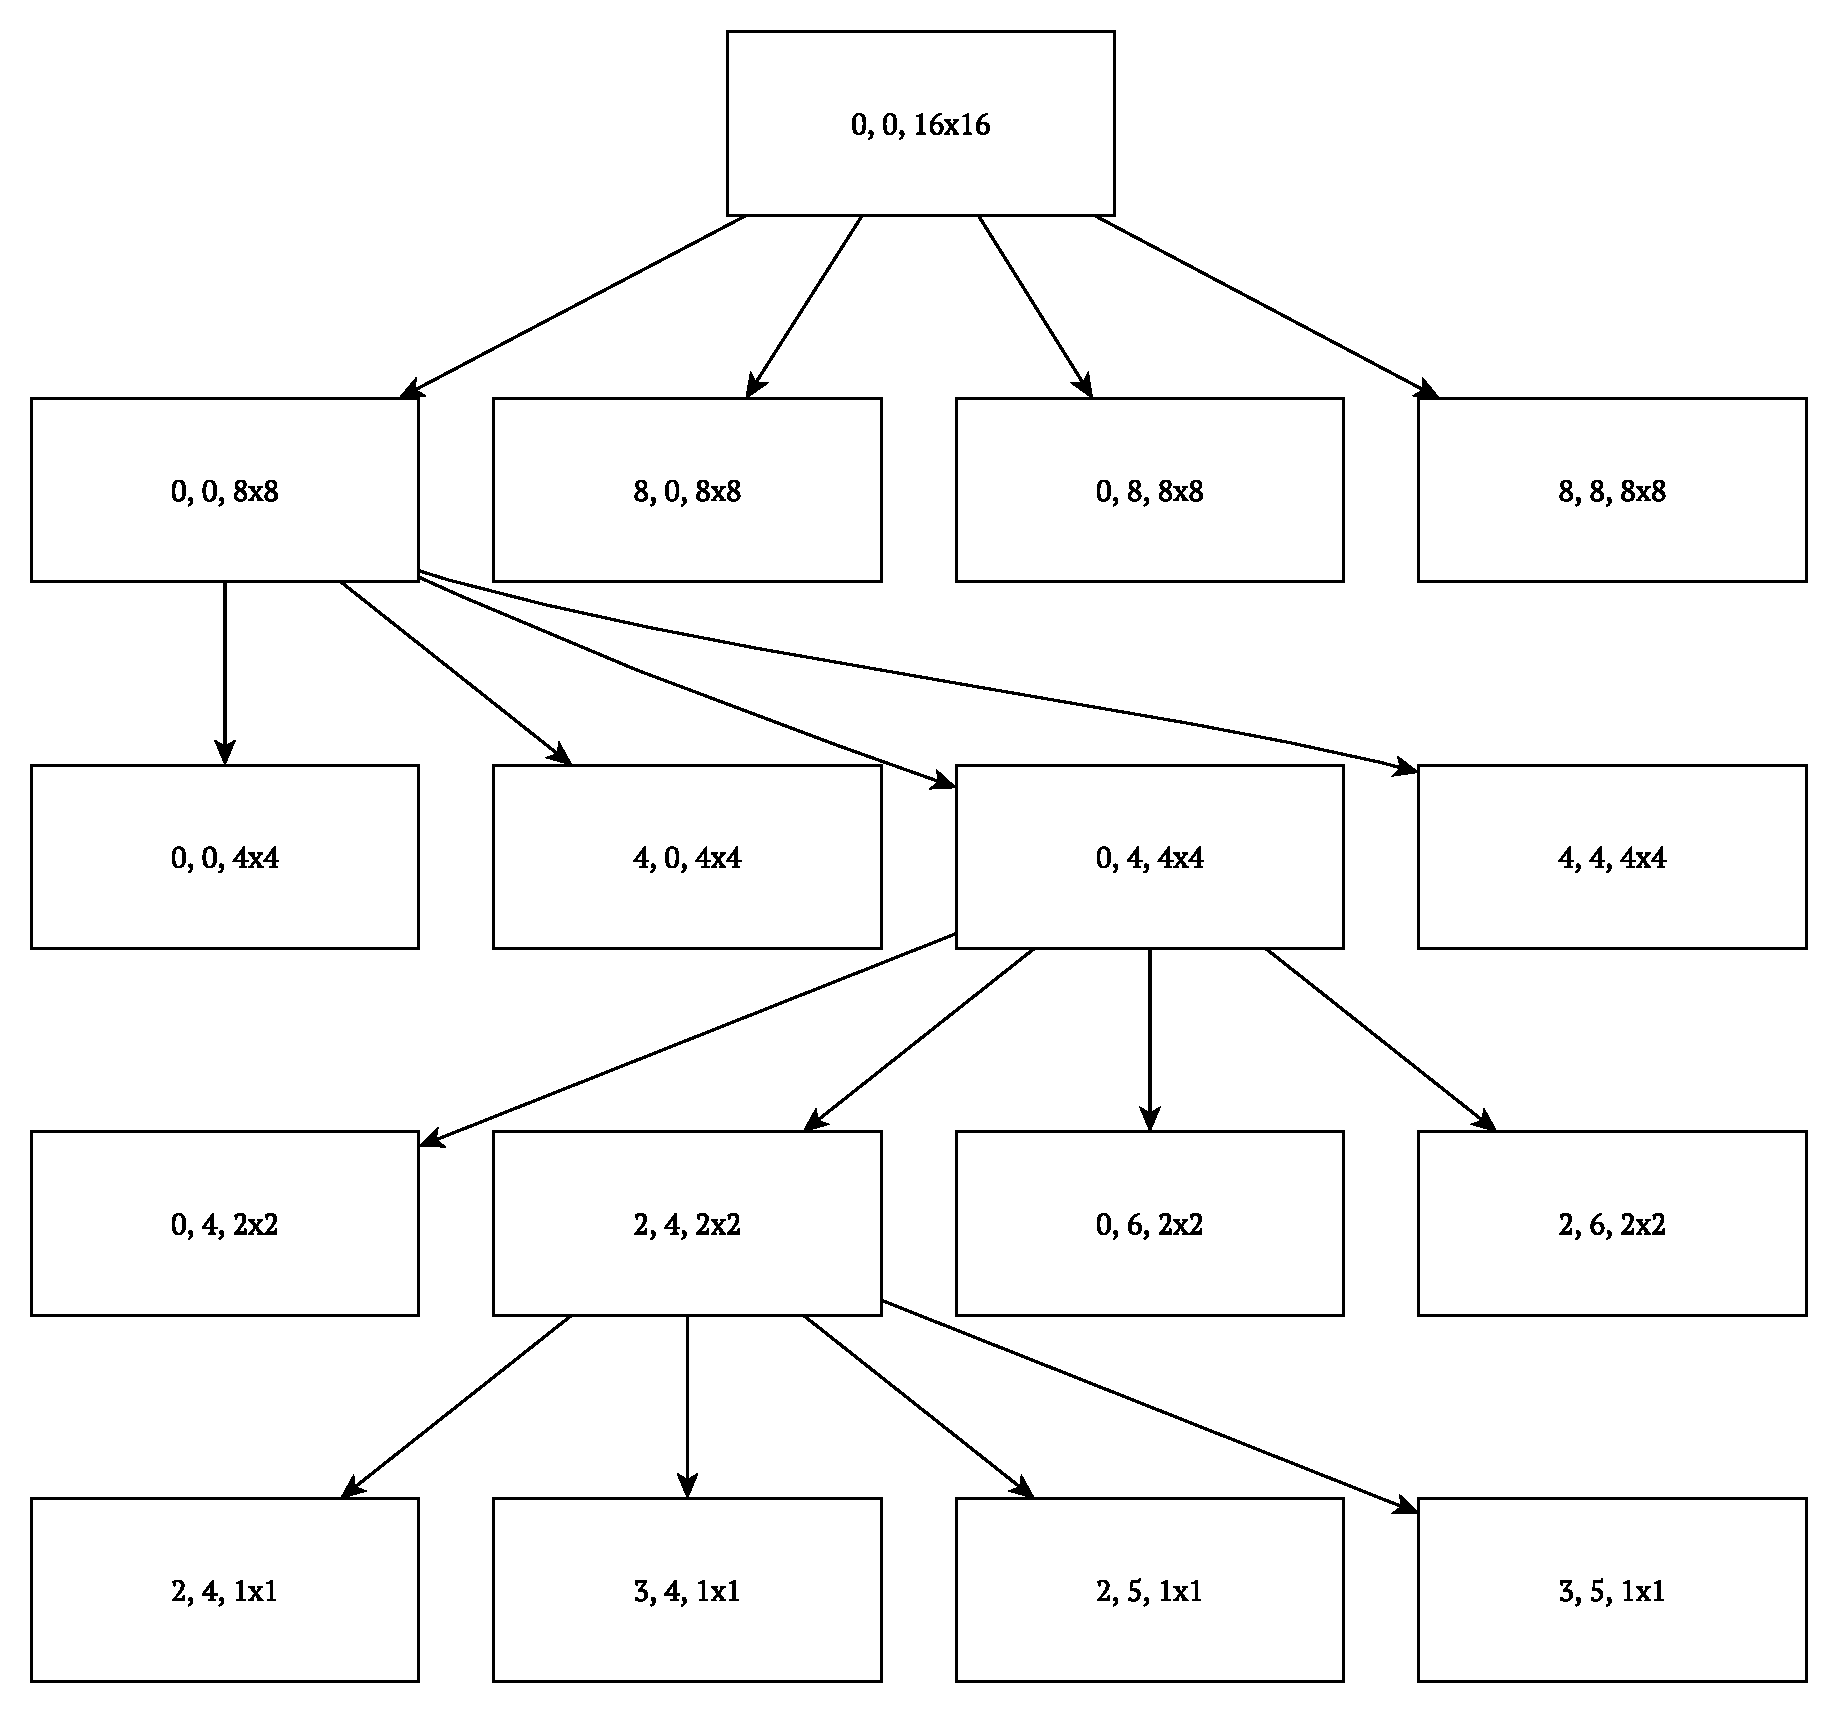
\includegraphics[width=0.85\linewidth]{windows.pdf}
    \caption{Дерево структуры подокон}
    \label{img:windows}
\end{figure}

На сложных сценах алгоритмы производят большое количество разбиений \cite{bib:8}. Алгоритмы требуют модификации для предоставления средств учета теней и освещения.

\subsubsection{Алгоритм, использующий z-буфер}

Идея алгоритма заключается в использовании буфера кадра и буфера глубины. Буфер кадра~---~буфер, в котором хранится информация о каждом пикселе изображения. Буфер глубины~---~буфер, в котором хранится информация о максимальной величине координаты $z$ отображаемого пиксела.

При обработке очередного многоугольника, для фиксированных $x$ и $y$ производится сравнение координаты $z$ со значением в буфере глубины, если оно больше, чем в буфере, то происходит обновление буфера кадра и буфера глубины с соответствующими значениями для текущего многоугольника.

В качестве особенностей алгоритма можно отметить его простоту, работу со сценами любой сложности, большой объем требуемой памяти \cite{bib:11}. Алгоритм требует модификации для предоставления средств учета теней и освещения.

\subsubsection{Алгоритмы построчного сканирования}

Идеей алгоритмов построчного сканирования является обработка сцены в порядке прохождения сканирующей строки. Такой подход позволяет перейти от трехмерной задачи удаления поверхностей к двумерной задаче удаления линий \cite{bib:12}.

Одним из вариантов алгоритма построчного сканирования является алгоритм построчного сканирования, использующий z-буфер. В отличие от классического алгоритма, при построчном сканировании нет необходимости хранить буфер кадра и буфер глубины для всего изображения, достаточно хранить буферы только для обрабатываемой строки. 

Таким образом, алгоритм построчного сканирования, использующий z-буфер требует меньший объем памяти, чем классический алгоритм. Алгоритмы требуют модификации для предоставления средств учета теней и освещения.


\subsubsection{Алгоритмы трассировки лучей}

В отличие от остальных алгоритмов, алгоритмы трассировки лучей, являются методами грубой силы, так как не учитывают специфику обрабатываемых объектов \cite{bib:8}. Идея алгоритмов заключается в отслеживании световых лучей между источниками света, объектами и наблюдателем. 

Алгоритм прямой трассировки лучей отслеживает лучи от источников света, с учетом их отражения от объектов сцены. Данный алгоритм является неэффективным \cite{bib:8}, так как множество лучей не доходят до наблюдателя, но все равно оказываются обработаны.

Альтернативой методу прямой трассировки является алгоритм обратной трассировки лучей, в котором происходит отслеживание световых лучей в обратном направлении, то есть от наблюдателя к объектам, от объектов к источникам света. Это позволяет обрабатывать только видимые наблюдателем лучи. Визуализация алгоритма приведена на рис.~\ref{img:raytracing}.

\noindent
\begin{figure}[h!]
	\centering
    \includegraphics[width=0.5\linewidth]{ray}
    \caption{Визуализация алгоритма обратной трассировки лучей}
    \label{img:raytracing}
\end{figure}

Алгоритмы позволяют учитывать тени и освещения, работают со сценами любой сложности. Кроме того, из-за присущей алгоритмам параллельности~---~лучи можно обрабатывать независимо друг от друга, алгоритм можно реализовывать с использованием методов параллельной обработки \cite{bib:9}.

\subsubsection{Выбор алгоритма удаления невидимых линий и поверхностей}
В рамках данной работы важен учет теней и освещения, кроме того, производится работа со сложными объектами~---~деревьями, так что необходимым является способность работы алгоритма работать со сценами любой сложности.

Кроме того, рассматривается возможность обработки сцены с использованием методов параллельной обработки. 

В соответствии с требованиями, для удаления невидимых линий и поверхностей был выбран алгоритм обратной трассировки лучей.


\subsection{Учет теней и освещения}
Так как для реализации удаления невидимых линий и поверхностей был выбран алгоритм обратной трассировки лучей, который позволяет учитывать тени и освещение, вопрос выбора методов учета теней и освещения в рамках данной работы не является актуальным.

\section{Генерация дерева}
Для генерации деревьев необходимо использовать следующее свойство: суммарная толщина веток, исходящих из некоторой другой ветки, равна толщине этой ветки \cite{bib:18}. Дерево в таком случае можно представить в виде графа \cite{bib:16}, а точнее~---~двоичного дерева, так как чаще всего ветка дерева разделяется на две части.

При получении питательных веществ, ветка увеличивается в размерах, причем если у нее нет потомков, то она увеличивается как в длину, так и в толщину. Если же у нее есть потомки, то происходит увеличение только в толщину, остальные питательные вещества переходят к потомкам.

При достижении веткой определенной длины, происходит ее разделение на две части, и рост этой ветки в длину прекращается.

\section{Выводы по аналитической части}
В данном разделе были формализованы объекты сцены, рассмотрены методы построения реалистичного изображения, методы хранения объектов, произведено сравнение существующих подходов. Был рассмотрен метод генерации деревьев.

\newpage